\preClass{Coordinate Systems}



\noindent Watch the Pre-Class videos for Section 3.3 and answer the following questions. Remember that in your written work you are graded on the correctness of your supporting work and not just your final answer. Always give an exact answer unless you are explicitly told to round; calculator approximations will not receive full credit. 


\begin{enumerate}
\item  Write the following in exponential form.
\begin{enumerate}
\item $\log_8(1)=0$
\vfill
\item $\ln(a)=b$
\vfill
\end{enumerate}


\item  Write the following in logarithmic form.
\begin{enumerate}
\item $7^0=1$
\vfill
\item $10^3=1000$
\vfill
\end{enumerate}

\item  Determine the domain of $\log_7(2x+5)$.  Write your answer in interval notation.
\vfill
\vfill

\newpage
\item  Graph the following functions.
\begin{enumerate}

\item Graph $\displaystyle f(x)=e^x$ along with it's asymptote.  (It is helpful to plot values for $x=0, 1, -1$.)\\
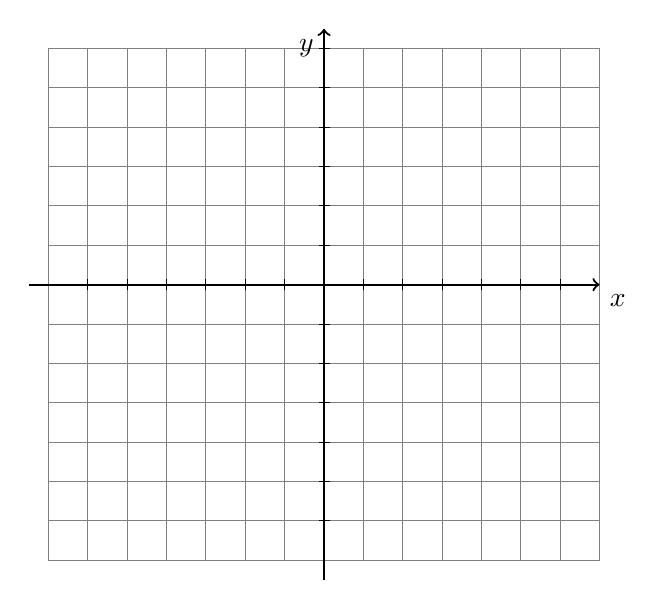
\begin{tikzpicture}[y=.5cm, x=0.5cm,font=\sffamily]
    %% ticks
    \draw[step = 1, gray] (-7,-7) grid (7,6);
    %% axis
    \draw[thick,->] (-7.5,0) -- coordinate (x axis mid) (7,0) node[anchor = north west] {$x$};
    \draw[thick,->] (0,-7.5) -- coordinate (y axis mid) (0,6.5) node[anchor = north east] {$y$};
    \foreach \y in {-6,-5,...,-1,1,2,...,6} {
      \draw (2pt, \y) -- (-2pt, \y);
    }
    \foreach \x in {-6,-5,...,-1,1,2,...,6} {
      \draw (\x,2pt) -- (\x,-2pt);
    }

\end{tikzpicture}



\item Use part $(a)$ to graph $\displaystyle g(x)=\ln(x)$ along with it's asymptote.\\

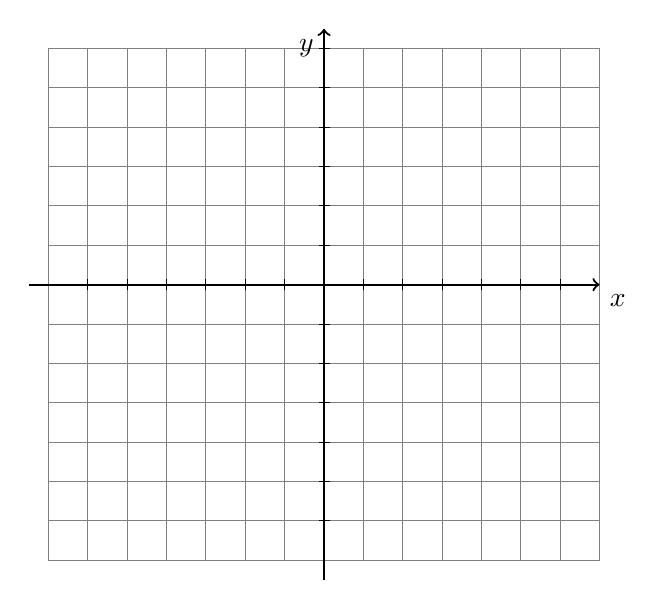
\begin{tikzpicture}[y=.5cm, x=0.5cm,font=\sffamily]
    %% ticks
    \draw[step = 1, gray] (-7,-7) grid (7,6);
    %% axis
    \draw[thick,->] (-7.5,0) -- coordinate (x axis mid) (7,0) node[anchor = north west] {$x$};
    \draw[thick,->] (0,-7.5) -- coordinate (y axis mid) (0,6.5) node[anchor = north east] {$y$};
    \foreach \y in {-6,-5,...,-1,1,2,...,6} {
      \draw (2pt, \y) -- (-2pt, \y);
    }
    \foreach \x in {-6,-5,...,-1,1,2,...,6} {
      \draw (\x,2pt) -- (\x,-2pt);
    }

\end{tikzpicture}


\vfill


\end{enumerate}






\end{enumerate}



